\documentclass[times, utf8, diplomski]{fer}
\usepackage{booktabs}
\usepackage{cite}
\usepackage{graphicx}
\usepackage{xcolor}

\graphicspath{ {./img/} }

\def\mat#1{\underline{#1}}
\def\TODO#1{\noindent\textcolor{red}{TODO: #1}\newline}

\begin{document}

\thesisnumber{1966}

\title{Optimizirane izlazne funkcije klasifikatora temeljenog na umjetnim neuronskim mrežama u domeni implementacijskih napada na kriptografske uređaje}

\author{Juraj Fulir}

\maketitle

% Ispis stranice s napomenom o umetanju izvornika rada. Uklonite naredbu \izvornik ako želite izbaciti tu stranicu.
\izvornik

\zahvala{ZAHVALA'n'STUFF}

\tableofcontents

\chapter{Uvod}
\TODO{ Opis problema }

\chapter{Implementacijski napadi na kriptografske uređaje}

\section{Side-channel napadi}
\TODO{ Postoji nekoliko vrsta.}
\TODO{ Ovdje se obrađuje DPA.}

\section{Izvedba napada}
\TODO{ Uštekaj uređaj, osciloskop na to i to mjesto i snimaj}
\TODO{ Provjeri mogućnosti i zaključi najvjerojatniju}
\TODO{ Problem netraktabilnosti postupka -> neuralke <3}

\section{DPA skupovi podataka}
\TODO{ Ima HW i ovaj pravi}
\TODO{ Nabaci i PCA redukcije i statistike iz jn}
\TODO{ Mjere dobrote klasifikacije}
\TODO{ Ne zaboravi referencu na stranicu!}

\chapter{Klasifikator temeljen na umjetnim neuronskim mrežama}

\section{Umjetne neuronske mreže}
Umjetne neuronske mreže (nadalje „neuronske mreže“) koristimo za modeliranje višedimenzijske funkcije ili distribucije kojom se aproksimira rješenje zadanog problema iz konačnog broja primjera. Vrlo su moćan alat za savladavanje teških zadataka u raznim područjima, često dostižući ljudske performanse na zadanom problemu. Danas su vrlo raširene u raznim područjima od kojih su samo neka: računalni vid \citep{alexnet,yolo}, prirodna obrada jezika \citep{word2vec,char_cnn} i podržano učenje \citep{atari,active_learn}.

\subsection{Građa}
Neuronske mreže građene su od međusobno povezanih jedinica, tzv. neurona, modeliranih prema pojednostavljenom modelu biološkog neurona. Neuron očitava ulazne značajke sustava ili izlaze drugih neurona te ažurira svoje unutarnje stanje (aktivaciju) i stvara odziv (izlaz). Utjecaj ulaza na neuron vrednuje se težinama \engl{weights} koje definiraju kako se neuron ponaša u ovisnosti o pojedinim ulazima. Aktivacijski prag neurona \engl{bias} određuje jedinstvenu osjetljivost neurona na jačinu podražaja. Težine i prag neurona nazivamo parametrima neurona.

\TODO{Što sve biolozi vele o neuronima? https://www.ncbi.nlm.nih.gov/pmc/articles/PMC3812748/}

\begin{figure}[h]
\centering
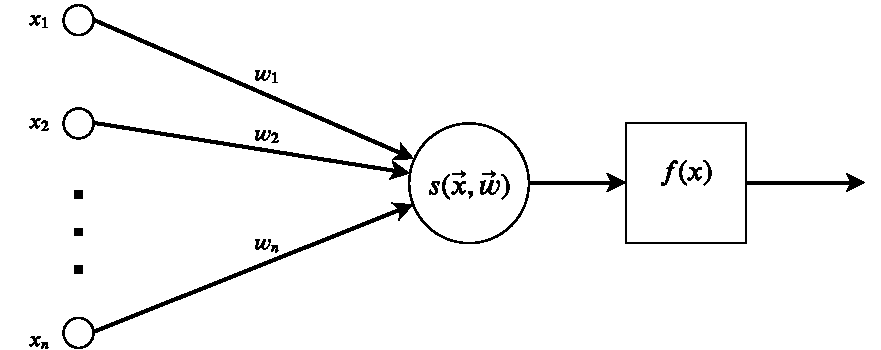
\includegraphics[scale=0.7]{Neuron.pdf}
\caption{Prikazani osnovni dijelovi neurona su težine dendrita ($w_i$), aktivacijska funkcija ($a(\vec{x},\vec{w})$) i izlazna funkcija ($f(x)$). Prag neurona nije prikazan zbog jednostavnosti dijagrama.}
\label{fig:neuron}
\end{figure}

Način na koji iz ulaza gradimo unutarnje stanje (aktivaciju) neurona opisujemo aktivacijskom funkcijom. Najpopularnije aktivacijske funkcije jesu afina funkcija i unakrsna korelacija.
Afina funkcija je skalarni produkt vektora ulaza s vektorom težina neurona uz dodatak vrijednosti praga. Parametri neurona definiraju nagib i pomak ravnine u prostoru ulaza koja opisuje aktivaciju neurona. Primijenjuje se kada se ulazi u model mogu zapisati vektorom značajki čiji raspored nije bitan.
\begin{equation}
f(\vec{x};\mat{W},\vec{b})=\mat{W}^T \cdot \vec{x} + \vec{b}
\end{equation}

\TODO{Spomeni distance based aktivacije (ANFIS?)}
\TODO{Spomeni i složenije metode: \citep{network_in_network}}

Pretvorbu aktivacije neurona u izlazni signal opisujemo izlaznom funkcijom koja se detaljnije obrađuje u poglavlju \ref{sec:izlazne_fje}. Aktivacijska i izlazna funkcija definiraju prijenosnu funkciju koja ujedno opisuje ponašanje cijelog neurona \citep{function_survey}. U praksi se pojam aktivacijske i prijenosne vrlo često ekvivalentno koristi na mjestu pojma izlazne funkcije, no ovaj rad se drži prethodno navedene i jasnije notacije.
\begin{equation}
t(x) = (f \circ a)(x) = f(a(x))
\end{equation}

Povezivanjem neurona gradi se arhitektura mreže koja određuje kako podatci i gradijenti teku kroz mrežu, a time utječu na brzinu učenja i inferencije neuronske mreže. Najčešće se koriste slojevite unaprijedne arhitekture zbog jednostavnosti izvedbe. Unaprijedne arhitekture propuštaju podatke samo u jednom smjeru odnosno već izračunati neuroni se ne izračunavaju ponovno, što je posebno pogodno za optimizaciju širenjem unatrag, detaljnije opisanu u poglavlju \ref{sec:backprop}. Slojevite arhitekture omogućuju paralelizaciju izvođenja operacija na grafičkim karticama što značajno ubrzava postupke učenja i inferencije. Pri definiciji slojevite arhitekture najčešće je dovoljno navesti samo redoslijed slojeva, no ponekad je potrebno definirati i način povezivanja slojeva npr. pri uporabi preskočnih veza \citep{highwaynet, resnet, densenet}. Prvi sloj služi za postavljanje ulaza mreže i nazivamo ga ulaznim slojem mreže. Posljednji sloj mreže služi nam za ekstrakciju izlaza te mjerenje kakvoće mreže i nazivamo ga izlaznim slojem mreže. Svi slojevi između ulaznog i izlaznog sloja nazivaju se skrivenim slojevima.

Potpuno povezana arhitektura je najjednostavnija arhitektura za zadatak klasifikacije. Svaki neuron u potpuno povezanom sloju aktivira se pomoću svih izlaza iz prethodnog sloja. Za naučeni potpuno povezani sloj kažemo da vrši ekstrakciju značajki iz svojih ulaza. Geometrijski gledano, svaki neuron vrši mapiranje značajki iz dimenzije prethodnog sloja u novu dimenziju s ciljem modeliranja boljih značajki.

Unakrsna korelacija, za razliku od afine funkcije, koristi informaciju o susjednosti ulaznih značajki. Ulaz za takav model je definiran n-dimenzijskim tenzorom, a neuron uzima samo jedan pod-tenzor ulaza (vidljiva regija) i nad njime računa skalarni produkt s n-dimenzijskim tenzorom težina (jezgrom). Kada su ulazi slike u boji ulazni tenzor ima 3 dimenzije (visina, širina, RGB kanali) pa stoga i jezgra ima 3 dimenzije, no znantno manje visine i širine. Unakrsna korelacija prozvana je konvolucijom jer radi na istom principu, a jedina razlika je da se elementi jezgre indeksiraju zrcaljeno po obje osi. S obzirom da se parametri jezgre uče automatski, nije nam bitno definirati orijentaciju jezgre.
\begin{equation}
f(\mat{X};\mat{W})=\mat{X} \circledast \mat{W}
\end{equation}

\TODO{Je li uopće potrebna konvolucija?}
\TODO{Raspisat konvoluciju po elementima?}

\subsection{Postupak optimizacije umjetne neuronske mreže}
Optimizacijom težina neuronska mreža prilagođava se danom zadatku, odnosno kažemo da mreža 'uči'. Optimizaciju težina najčešće izvodimo gradijentnim spustom, uz pretpostavku derivabilnosti svih komponenata neuronske mreže. Kada ta pretpostavka ne vrijedi koriste se algoritmi pretrage poput evolucijskih algoritama. U ovom radu optimizacija se vrši gradijentnim spustom.

\subsubsection{Inicijalizacija težina}
* važnost dobre inicijalizacije
[slika dobre i loše inicijalizacije]
* Xavier

\subsection{Funkcija gubitka}

\subsection{Optimizacija širenjem unatrag}
\label{sec:backprop}

\subsubsection{Optimizator}
* geometrijski značaj optimizacije
[slika podnaučena, generalizira, prenaučena]

\subsubsection{Perturbacije ulaznih podataka}

\subsection{Svojstva}
* Svojstva kompresije, generalizacije, univerzalne aproksimacije


\subsection{Problemi}
* Problem odabira arhitekture, hiperparametara i optimizacije
* Problem pretreniranosti + adversarial primjeri

Arhitektura, prijenosne funkcije i težine definiraju neuronsku mrežu te njihov odabir značajno utjeće na performanse neuronske mreže. Učenje 

Derivabilne neuronske mreže optimiziraju se optimizatorom koji određuje kako se mijenjaju težine.Za ugađanje težina najčešće se koristi gradijentni spust, uz pretpostavku derivabilnosti čitave neuronske mreže. Kada pretpostavka ne vrijedi najčešće se koriste evolucijski algoritmi.

\section{Izlazne funkcije}
\label{sec:izlazne_fje}
\TODO{Bitka za odabir izlazne fje (nađi onaj rad di pljuje po sigmoidi i relu (elu rad?))}
\TODO{Usporedbe funkcije i derivacije}
\TODO{Navedene su funkcije koje su razmatrane}

\subsection*{Ispravljena linearna jedinica (ReLU)}
\engl{Rectified linear unit}
* bez i sa cutoff

\begin{equation}
\begin{split}
f(x) = 
\begin{cases}
x,		& \text{ako } x > 0 \\
0,		& \text{inače}
\end{cases}
\end{split}
\qquad
\begin{split}
f'(x) = 
\begin{cases}
1,		& \text{ako } x > 0 \\
0,		& \text{inače}
\end{cases}
\end{split}
\end{equation}

\subsection*{Propusna ispravljena linearna jedinica (LReLU)}
\engl{Leaky ReLU}

\begin{equation}
\begin{split}
f(x) = 
\begin{cases}
x,			& \text{ako } x > 0 \\
\alpha x,	& \text{inače}
\end{cases}
\end{split}
\qquad
\begin{split}
f'(x) = 
\begin{cases}
1,		& \text{ako } x > 0 \\
\alpha,	& \text{inače}
\end{cases}
\end{split}
\end{equation}

\subsection*{Ispravljena linearna jedinica s pragom (ThReLU)}
\engl{Thresholded ReLU}

\begin{equation}
\begin{split}
f(x) = 
\begin{cases}
x,		& \text{ako } x > \theta \\
0,		& \text{inače}
\end{cases}
\end{split}
\qquad
\begin{split}
f'(x) = 
\begin{cases}
1,		& \text{ako } x > \theta \\
0,		& \text{inače}
\end{cases}
\end{split}
\end{equation}

\subsection*{(RReLU)}

\subsection*{Eksponencijalno-linearna jedinica (ELU)}
\engl{Exponential linear unit}

\begin{equation}
\begin{split}
f(x) = 
\begin{cases}
x,					& \text{ako } x > 0 \\
\alpha (e^x - 1),	&  \text{inače}
\end{cases}
\end{split}
\qquad
\begin{split}
f'(x) = 
\begin{cases}
1,	 		& \text{ako } x > 0 \\
\alpha e^x,	& \text{inače}
\end{cases}
\end{split}
\end{equation}

\subsection*{Skalirana eksponencijalno-linearna jedinica (SELU)}
\engl{Scaled exponential linear unit}

\begin{equation}
\begin{split}
f(x) = \lambda
\begin{cases}
x,					& \text{ako } x > 0 \\
\alpha (e^x - 1),	&  \text{inače}
\end{cases}
\end{split}
\qquad
\begin{split}
f'(x) = \lambda
\begin{cases}
1,	 		& \text{ako } x > 0 \\
\alpha e^x,	& \text{inače}
\end{cases}
\end{split}
\end{equation}

\subsection*{(GELU)}

\subsection*{Sigmoida ($\sigma $)}
\engl{Sigmoid}

\begin{equation}
\begin{split}
f(x) = \frac{1}{1+e^{-x}}
\end{split}
\qquad
\begin{split}
f'(x) = \sigma(x)(1-\sigma(x))
\end{split}
\end{equation}

\subsection*{Tvrda sigmoida}
\engl{Hard sigmoid}

\begin{equation}
\begin{split}
f(x) = min(1,\ max(0,\ 0.2x + 0.5))
\end{split}
\qquad
\begin{split}
f'(x) = 
\begin{cases}
0.2,	 		& \text{ako } x \in [-2.5, 2.5] \\
0,	& \text{inače}
\end{cases}
\end{split}
\end{equation}

\subsection*{Swish}
\begin{equation}
\begin{split}
f(x) = x \sigma(\beta x)
\end{split}
\qquad
\begin{split}
f'(x) &= \sigma(\beta x) + \beta x \cdot \sigma(\beta x)(1-\sigma(\beta x)) \\
&= \frac{e^x \cdot (e^x + x + 1)}{(e^x + 1)^2}
\end{split}
\end{equation}

\subsection*{Tangens hiperbolni (tanh)}

\begin{equation}
\begin{split}
f(x) = \frac{e^x - e^{-x}}{e^x + e^{-x}}
\end{split}
\qquad
\begin{split}
f'(x) = 1 - tanh^2(x)
\end{split}
\end{equation}

\subsection*{Tvrdi tangens hiperbolni}
\engl{Hard tanh}

\begin{equation}
\begin{split}
f(x) =
\begin{cases}
-1,	 		& \text{ako } x < 1 \\
x,	 		& \text{ako } x \in [-1,1] \\
1,	& \text{inače}
\end{cases}
\end{split}
\qquad
\begin{split}
f'(x) =
\begin{cases}
0,	 		& \text{ako } x < 1 \\
1,	 		& \text{ako } x \in [-1,1] \\
0,	& \text{inače}
\end{cases}
\end{split}
\end{equation}

\subsection*{Racionalna aproksimacija tanh}
\engl{Rational tanh}
??????????????????
\begin{equation}
f(x) = 1.7159 \cdot tanh(\frac{2}{3}x)\text{,\quad gdje }
tanh(x) \approx sgn(x)(1 - \frac{1}{1 + |x| + x^2 + 1.41645 \cdot x^4}) \\
f'(x) =
\end{equation}

\subsection*{Ispravljeni tanh}
\engl{Rectified tanh}

\subsection*{Softmax}
\begin{equation}
\begin{split}
f(\vec{x}) = \frac{e^{\vec{x}}}{\sum_ie^{\vec{x_i}}}
\end{split}
\qquad
\begin{split}
f'(x) = \frac{e^x}{1+e^x}
\end{split}
\end{equation}

\subsection*{Softplus}
\begin{equation}
\begin{split}
f(x) = log(1+e^x)
\end{split}
\qquad
\begin{split}
f'(x) = \frac{e^x}{1+e^x}
\end{split}
\end{equation}

\subsection*{Softsign}
\begin{equation}
\begin{split}
f(x) = \frac{x}{1+|x|}
\end{split}
\qquad
\begin{split}
f'(x) = \frac{1}{(1+|x|)^2}
\end{split}
\end{equation}

\subsection*{Sinus (sin)}
\begin{equation}
\begin{split}
f(x) = sin(x)
\end{split}
\qquad
\begin{split}
f'(x) = cos(x)
\end{split}
\end{equation}

\subsection*{Kosinus (cos)}
\begin{equation}
\begin{split}
f(x) = cos(x)
\end{split}
\qquad
\begin{split}
f'(x) = -sin(x)
\end{split}
\end{equation}

\subsection*{Parabola $x^2$}
\begin{equation}
\begin{split}
f(x) = x^2
\end{split}
\qquad
\begin{split}
f'(x) = 2x
\end{split}
\end{equation}

\subsection*{Kubna parabola $x^3$}
\begin{equation}
\begin{split}
f(x) = x^3
\end{split}
\qquad
\begin{split}
f'(x) = 3x^2
\end{split}
\end{equation}

\subsection*{Gauss}
\begin{equation}
\begin{split}
f(x) = e^{-x^2}
\end{split}
\qquad
\begin{split}
f'(x) = -2x \cdot f(x)
\end{split}
\end{equation}

\chapter{Optimizacija simboličkom regresijom (tehnički genetskim programiranjem...)}

\section{Simbolička regresija}
* Opis i svojstva SR
* Utjecaj i brojnost parametara u GA (moš linkat i svoj završni rad :P)

\section{Taboo evolucijski algoritam}
* Problem konvergencije i stohastičnosti GP-a
* EA oplemenjen taboo listom iz algoritma Taboo pretraživanja

\section{Korišteni čvorovi i operatori (prostor pretraživanja)}
* Popis čvorova
* Popis operatora (un/bin)

\chapter{Implementacija}
???

\chapter{Rezultati}

\section{9class}

\subsection{Uobičajene izlazne funkcije}
* Opis postupka pretrage
* Tablica
* Komentar

\subsection{Utjecaj parametra veličine taboo liste}
* Tablica
* Komentar

\section{256class}

\subsection{Uobičajene izlazne funkcije}
* Opis postupka pretrage
* Tablica
* Komentar

\subsection{Utjecaj parametra veličine taboo liste}
* Tablica
* Komentar

\chapter{Buduća istraživanja}
* Primjena CNN na vremenskim uzorcima po uzoru na onaj rad
* Ispitivanje učinkovitosti korištene optimizacije na ostalim problemima
* Paralelna evolucija arhitekture i aktivacijskih fja

\chapter{Zaključak}
* Radi/Ne radi. 
* Pronađene zanimljivosti. 
* Pouka za doma.

\bibliography{literatura}
\bibliographystyle{fer}

\begin{sazetak}
Proučiti postojeće metode u izgradnji izlaznih funkcija u umjetnim neuronskim mrežama. Posebnu pažnju posvetiti evolucijskim algoritmima simboličke regresije za izgradnju ciljanih funkcija. Ustanoviti moguće nedostatke postojećih algoritama ili mogućnost poboljšanja. Primijeniti evoluirane izlazne funkcije u homogenoj ili heterogenoj umjetnoj neuronskoj mreži na skupovima DPAv2 i DPAv4 te odrediti mjere kvalitete izgrađenog klasifikatora: točnost, preciznost, odziv te F mjere. Usporediti učinkovitost ostvarenih postupaka s postojećim rješenjima iz literature. Radu priložiti izvorne tekstove programa, dobivene rezultate uz potrebna objašnjenja i korištenu literaturu.

\kljucnerijeci{Ključne riječi, odvojene zarezima.}
\end{sazetak}

% TODO: Navedite naslov na engleskom jeziku.
\engtitle{Title}
\begin{abstract}
Abstract.

\keywords{Keywords.}
\end{abstract}

\end{document}
